\documentclass[presentation]{beamer}
\mode<presentation>{\usetheme{AMSBolognaFCrev}}

\usepackage[utf8]{inputenc}
\usepackage[T1]{fontenc}
\usepackage{booktabs}
\usepackage{array}
\usepackage{colortbl}
\usepackage{tikz}
\usepackage[ddmmyyyy]{datetime}
\usepackage[export]{adjustbox}
\usetikzlibrary{arrows.meta,positioning,shapes.geometric}

\renewcommand{\dateseparator}{/}
\newcommand{\sectiontitleframe}[1]{
\begin{frame}[plain,c]
\begin{center}
{\usebeamerfont{title}\usebeamercolor[fg]{title}#1}
\end{center}
\end{frame}
}

\title[Lesson 3]{Access Control in Healthcare Systems}
\institute[Data Privacy and Security]{Healthcare Data Privacy and Security}
\author[\sspeaker{G. Pisano}]{\speaker{Giuseppe Pisano} \\\href{mailto:g.pisano@unibo.it}{g.pisano@unibo.it}}
\date[August, 2026]{August, 2026}
%
\titlegraphic{
%\vspace{0.2cm}
\begin{center}
    
\includegraphics[width=0.35\textwidth, valign=c]{logos/intestazione.png}
    
\includegraphics[width=0.16\textwidth, valign=c]{logos/unibo_logo_2.png}
    
\includegraphics[width=0.11\textwidth, valign=c]{logos/makeni_logo_2.png}
    
\includegraphics[width=0.20\textwidth, valign=c]{logos/cuamm_logo_png.png}
\end{center}
\centering
\tiny{S.K.I.L.L.E.D --- AID013244/04/2\\Strategic Knowledge and Inclusive Lifelong Learning in the health sector for youth Employability and Development}
}

\begin{document}

\setbeamertemplate{frametitle}
{
    \nointerlineskip
    \begin{beamercolorbox}[sep=0.3cm,ht=2.2em,wd=\paperwidth]{frametitle}
        \vbox{}\vskip-2ex%
        \strut\insertframetitle\hfill\raisebox{-0.2\height}{
\includegraphics[width=2cm]{logos/cuamm_logo_png.png}}\strut
        \vskip-0.8ex%
    \end{beamercolorbox}
}

\begin{frame}[allowframebreaks]
\titlepage
\end{frame}

\begin{frame}[c,allowframebreaks]{Roadmap}
\tableofcontents[hideallsubsections]
\end{frame}

\begin{frame}[c]{How This Lesson Progresses}
\begin{block}{Learning path}
We move from the \textbf{purpose} of access control, to the \textbf{decision flow}, then to
\textbf{policies}, \textbf{subjects and objects}, and finally to the main access-control models:
\textbf{DAC}, \textbf{MAC}, and \textbf{RBAC}.
\end{block}

\begin{exampleblock}{Hospital storyline}
We continue with St. Isidore Hospital. A doctor, nurse, lab technician, billing clerk, system
administrator, medical device, and external specialist all need access, but not to the same data,
not with the same actions, and not in every circumstance.
\end{exampleblock}
\end{frame}

\begin{frame}[c]{Connection with Other Lessons}
\begin{block}{Where this fits}
Access control turns security goals into operational decisions: \textbf{who} can do \textbf{what},
to \textbf{which resource}, under \textbf{which conditions}, and with \textbf{which traceability}.
\end{block}

\begin{itemize}
    \item \textbf{Basic networking}: access decisions protect services exposed on the network.
    \item \textbf{Encryption}: access control decides who may use keys and decrypt data.
    \item \textbf{Authentication}: identity evidence comes before authorization.
    \item \textbf{GDPR}: access must support confidentiality, accountability, minimization, and auditability.
\end{itemize}
\end{frame}

\section{Access Control Purpose}
\sectiontitleframe{Access Control Purpose}

\begin{frame}[c]{Section Context: Access Control Purpose}
\begin{block}{What we are talking about}
Access control is the security function that mediates every attempt to use a protected resource.
It prevents unauthorized use, but also prevents \textbf{misuse by authorized users}.
\end{block}

\begin{exampleblock}{Hospital lens}
A cardiologist may be authorized to open the EHR, but that does not mean they may export every
patient record, alter medication orders outside their ward, or read celebrity patient files out of
curiosity.
\end{exampleblock}
\end{frame}

\begin{frame}[c]{Definition}
\begin{block}{Core idea}
Access control implements a security policy specifying \textbf{who or what} may access a system
resource, \textbf{which operation} is allowed, and \textbf{under which circumstances}
\cite{rfc4949}.
\end{block}

\begin{exampleblock}{Hospital example}
The patient portal allows a patient to read their own lab results. It does not allow that patient to
read another patient's discharge summary or modify the physician's diagnosis.
\end{exampleblock}
\end{frame}

\begin{frame}[c]{Three Goals}
\begin{block}{Access control should}
\begin{itemize}
    \item block access by \textbf{unauthorized} subjects;
    \item stop \textbf{authorized} subjects from using resources in unauthorized ways;
    \item allow legitimate users to complete legitimate work.
\end{itemize}
\end{block}

\begin{exampleblock}{Hospital example}
A nurse on the surgical ward should be able to update vital signs for assigned patients, but not
change radiology reports or browse psychiatric notes for unrelated patients.
\end{exampleblock}
\end{frame}

\begin{frame}[c]{Why It Is Central}
\begin{block}{Security as mediation}
Many security mechanisms eventually support an access decision. Firewalls mediate network flows;
operating systems mediate files and processes; databases mediate records and fields; applications
mediate business actions.
\end{block}

\begin{exampleblock}{Hospital example}
The same access-control question appears when a clinician logs into the EHR, when a pharmacy
system receives a medication order, and when a backup server reads encrypted database snapshots.
\end{exampleblock}
\end{frame}

\begin{frame}[c]{Scheme: Access Request}
\begin{center}
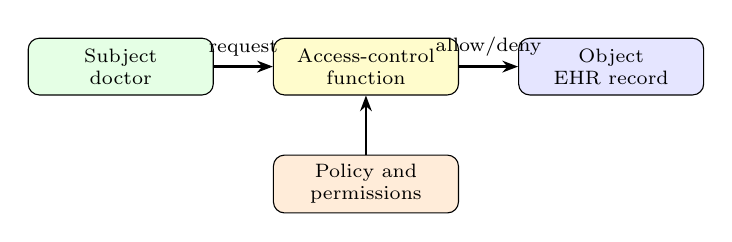
\begin{tikzpicture}[
    node distance=0.75cm,
    box/.style={draw, rounded corners, align=center, minimum width=2.35cm, minimum height=0.72cm, font=\scriptsize},
    link/.style={-{Stealth[length=2mm]}, thick}
]
\node[box, fill=green!10] (subject) {Subject\\doctor};
\node[box, right=of subject, fill=yellow!20] (control) {Access-control\\function};
\node[box, right=of control, fill=blue!10] (object) {Object\\EHR record};
\node[box, below=of control, fill=orange!15] (policy) {Policy and\\permissions};
\draw[link] (subject) -- node[above,font=\scriptsize]{request} (control);
\draw[link] (control) -- node[above,font=\scriptsize]{allow/deny} (object);
\draw[link] (policy) -- (control);
\end{tikzpicture}
\end{center}

\begin{block}{Reading the scheme}
The user does not access the resource directly. A trusted mediation point evaluates the request
against policy before the operation is executed.
\end{block}
\end{frame}

\begin{frame}[c]{Recap: Access Control Purpose}
\begin{block}{Takeaways}
\begin{itemize}
    \item Access control is about \textbf{authorized use}, not only login.
    \item The decision combines subject, object, operation, and context.
    \item In healthcare, correct access is also a patient-safety requirement.
\end{itemize}
\end{block}
\end{frame}

\section{Authentication, Authorization, Audit}
\sectiontitleframe{Authentication, Authorization, Audit}

\begin{frame}[c]{Section Context: AAA}
\begin{block}{What we are talking about}
Access control depends on three related functions: \textbf{authentication}, \textbf{authorization},
and \textbf{audit}. They answer different questions and should not be confused.
\end{block}

\begin{exampleblock}{Hospital lens}
The hospital first checks that ``Dr. Rossi'' is really Dr. Rossi. Then it checks whether that role
may prescribe for this patient. Later, audit logs allow review of what happened.
\end{exampleblock}
\end{frame}

\begin{frame}[c]{Authentication}
\begin{block}{Question}
\textbf{Authentication} verifies that the entity presenting credentials is who or what it claims to
be.
\end{block}

\begin{exampleblock}{Hospital example}
A doctor uses a password plus a smart card. A medication dispensing cabinet authenticates itself to
the pharmacy server using a device certificate.
\end{exampleblock}
\end{frame}

\begin{frame}[c]{Authorization}
\begin{block}{Question}
\textbf{Authorization} determines which permissions the authenticated entity has for a requested
resource and operation.
\end{block}

\begin{exampleblock}{Hospital example}
After login, the EHR checks whether the doctor has an active care relationship with the patient and
whether prescribing is allowed for that department.
\end{exampleblock}
\end{frame}

\begin{frame}[c]{Audit}
\begin{block}{Question}
\textbf{Audit} independently records and reviews security-relevant activity to test whether controls
are adequate and whether behavior matches policy.
\end{block}

\begin{exampleblock}{Hospital example}
The privacy office reviews accesses to VIP patient records and flags staff members who opened
records without a treatment, payment, or operations reason.
\end{exampleblock}
\end{frame}

\begin{frame}[c]{Scheme: AAA Flow}
\begin{center}
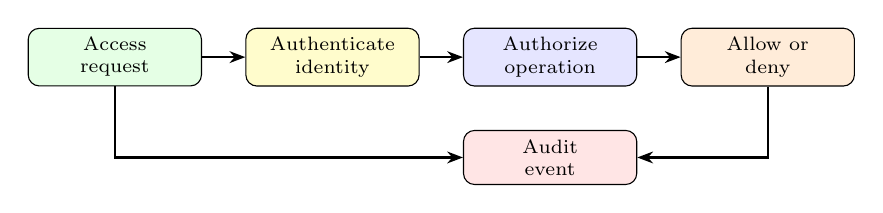
\begin{tikzpicture}[
    node distance=0.55cm,
    box/.style={draw, rounded corners, align=center, minimum width=2.2cm, minimum height=0.65cm, font=\scriptsize},
    link/.style={-{Stealth[length=2mm]}, thick}
]
\node[box, fill=green!10] (request) {Access\\request};
\node[box, right=of request, fill=yellow!20] (authn) {Authenticate\\identity};
\node[box, right=of authn, fill=blue!10] (authz) {Authorize\\operation};
\node[box, right=of authz, fill=orange!15] (decision) {Allow or\\deny};
\node[box, below=of authz, fill=red!10] (audit) {Audit\\event};
\draw[link] (request) -- (authn);
\draw[link] (authn) -- (authz);
\draw[link] (authz) -- (decision);
\draw[link] (request) |- (audit);
\draw[link] (decision) |- (audit);
\end{tikzpicture}
\end{center}

\begin{block}{Important}
Authentication alone is not enough. A valid identity can still request an operation that policy
does not allow.
\end{block}
\end{frame}

\begin{frame}[c]{Recap: AAA}
\begin{block}{Takeaways}
\begin{itemize}
    \item Authentication proves identity or device legitimacy.
    \item Authorization decides permitted actions.
    \item Audit creates accountability and supports incident investigation.
    \item Strong systems keep these functions connected but conceptually separate.
\end{itemize}
\end{block}
\end{frame}

\section{Policy Design Principles}
\sectiontitleframe{Policy Design Principles}

\begin{frame}[c]{Section Context: Policy Design Principles}
\begin{block}{What we are talking about}
A policy is not only a table of permissions. It also defines assumptions, defaults, delegation
rules, conflict handling, and administrative power.
\end{block}

\begin{exampleblock}{Hospital lens}
Bad policy design can either block urgent care or expose sensitive data. The goal is controlled
flexibility: enough access for care, enough restriction for privacy and safety.
\end{exampleblock}
\end{frame}

\begin{frame}[c]{Reliable Input}
\begin{block}{Concept}
Access control assumes that the inputs used for decisions are reliable: identity, role, device,
location, time, patient relationship, and requested operation.
\end{block}

\begin{exampleblock}{Hospital example}
If the EHR trusts a forged department value, an attacker could make a normal account appear to be
part of the intensive-care unit. Reliable identity and context data are part of the control.
\end{exampleblock}
\end{frame}

\begin{frame}[c]{Fine-Grained and Coarse-Grained Rules}
\begin{block}{Concept}
Policies may be coarse-grained, such as access to an application, or fine-grained, such as access
to a single field in a record. Real systems usually need both.
\end{block}

\begin{exampleblock}{Hospital example}
A billing clerk may open the patient account but should not see psychotherapy notes. A physician
may see clinical notes but not modify billing codes.
\end{exampleblock}
\end{frame}

\begin{frame}[c]{Least Privilege}
\begin{block}{Concept}
\textbf{Least privilege} means granting only the permissions needed for the current task
\cite{saltzer1975protection}.
\end{block}

\begin{exampleblock}{Hospital example}
A temporary radiology intern receives read access to imaging studies for assigned patients, not
administrator access to the PACS database.
\end{exampleblock}
\end{frame}

\begin{frame}[c]{Separation of Duty}
\begin{block}{Concept}
\textbf{Separation of duty} divides sensitive authority across multiple people or roles so that one
person cannot complete a dangerous action alone.
\end{block}

\begin{exampleblock}{Hospital example}
One administrator requests creation of a high-privilege EHR account, but a different administrator
must approve it before the account becomes active.
\end{exampleblock}
\end{frame}

\begin{frame}[c]{Open and Closed Policies}
\begin{block}{Two defaults}
An \textbf{open policy} permits access unless a rule denies it. A \textbf{closed policy} denies
access unless a rule permits it.
\end{block}

\begin{exampleblock}{Hospital example}
For clinical records, St. Isidore uses a closed default: no staff member sees a patient file unless
a role, assignment, or break-glass emergency rule permits it.
\end{exampleblock}
\end{frame}

\begin{frame}[c]{Policy Conflicts}
\begin{block}{Concept}
Multiple policies may apply to the same resource. A system must define how conflicts are resolved:
for example, whether deny rules override allow rules.
\end{block}

\begin{exampleblock}{Hospital example}
A doctor is part of the cardiology team, but a special privacy restriction marks a patient record as
sensitive. The EHR needs a clear conflict rule before deciding access.
\end{exampleblock}
\end{frame}

\begin{frame}[c]{Administrative Policies and Dual Control}
\begin{block}{Concept}
Administrative policies specify who may add, remove, or modify permissions. \textbf{Dual control}
requires two or more people to approve especially sensitive actions.
\end{block}

\begin{exampleblock}{Hospital example}
Changing the emergency department's access rules requires approval from both IT security and the
clinical governance lead.
\end{exampleblock}
\end{frame}

\begin{frame}[c]{Scheme: Policy Evaluation}
\begin{center}
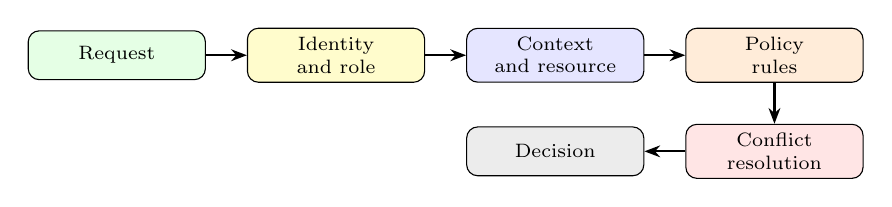
\begin{tikzpicture}[
    node distance=0.52cm,
    box/.style={draw, rounded corners, align=center, minimum width=2.25cm, minimum height=0.62cm, font=\scriptsize},
    link/.style={-{Stealth[length=2mm]}, thick}
]
\node[box, fill=green!10] (req) {Request};
\node[box, right=of req, fill=yellow!20] (id) {Identity\\and role};
\node[box, right=of id, fill=blue!10] (ctx) {Context\\and resource};
\node[box, right=of ctx, fill=orange!15] (rules) {Policy\\rules};
\node[box, below=of rules, fill=red!10] (conflict) {Conflict\\resolution};
\node[box, left=of conflict, fill=gray!15] (decision) {Decision};
\draw[link] (req) -- (id);
\draw[link] (id) -- (ctx);
\draw[link] (ctx) -- (rules);
\draw[link] (rules) -- (conflict);
\draw[link] (conflict) -- (decision);
\end{tikzpicture}
\end{center}

\begin{block}{Reading the scheme}
Policy evaluation is a chain. Weak input, unclear rules, or undefined conflicts can all produce
unsafe access decisions.
\end{block}
\end{frame}

\begin{frame}[c]{Recap: Policy Design Principles}
\begin{block}{Takeaways}
\begin{itemize}
    \item Least privilege limits blast radius.
    \item Separation of duty and dual control reduce abuse of sensitive powers.
    \item Closed policies are usually safer for clinical and personal data.
    \item Conflict rules and administrative rules are part of the policy.
\end{itemize}
\end{block}
\end{frame}

\section{Subjects, Objects, and Rights}
\sectiontitleframe{Subjects, Objects, and Rights}

\begin{frame}[c]{Section Context: Subjects, Objects, and Rights}
\begin{block}{What we are talking about}
Before comparing access-control models, we need the vocabulary used by all of them:
\textbf{subjects}, \textbf{objects}, and \textbf{access rights}.
\end{block}

\begin{exampleblock}{Hospital lens}
The same person may act as different subjects at different times: a physician in a clinical role, a
researcher in a research role, or an administrator in a maintenance role.
\end{exampleblock}
\end{frame}

\begin{frame}[c]{Subjects}
\begin{block}{Concept}
A \textbf{subject} is an active entity that requests access to an object. It may be a user, process,
service, device, or application.
\end{block}

\begin{exampleblock}{Hospital example}
Subjects include a nurse using the EHR, a lab analyzer sending results, a backup service reading
database files, and an API gateway calling the patient portal.
\end{exampleblock}
\end{frame}

\begin{frame}[c]{Owner, Group, World}
\begin{block}{Common classes}
Many systems organize subjects into \textbf{owner}, \textbf{group}, and \textbf{world}. The owner
has special control, groups collect shared permissions, and world represents everyone else.
\end{block}

\begin{exampleblock}{Hospital example}
A discharge-template file may be owned by the clinical documentation lead, writable by the
documentation team, and readable by all clinicians.
\end{exampleblock}
\end{frame}

\begin{frame}[c]{Objects}
\begin{block}{Concept}
An \textbf{object} is a protected resource that contains, receives, or controls information.
\end{block}

\begin{exampleblock}{Hospital example}
Objects include EHR records, lab results, PACS images, medication orders, audit logs, API
endpoints, database tables, report files, and device configuration screens.
\end{exampleblock}
\end{frame}

\begin{frame}[c]{Access Rights}
\begin{block}{Concept}
An \textbf{access right} describes the operation a subject may perform on an object.
\end{block}

\begin{itemize}
    \item \textbf{Read}: view or copy information.
    \item \textbf{Write}: add or modify information.
    \item \textbf{Execute}: run a program or invoke an operation.
    \item \textbf{Delete}: remove an object.
    \item \textbf{Create}: make a new object.
    \item \textbf{Search}: list or discover objects.
\end{itemize}
\end{frame}

\begin{frame}[c]{Rights Need Context}
\begin{block}{Important}
The meaning of a right depends on the object. ``Write'' on a note, ``write'' on a medication
order, and ``write'' on an audit log have very different risk.
\end{block}

\begin{exampleblock}{Hospital example}
A nurse may write vital signs. Only a prescriber may write medication orders. Almost nobody should
write audit logs directly.
\end{exampleblock}
\end{frame}

\begin{frame}[c]{Recap: Subjects, Objects, and Rights}
\begin{block}{Takeaways}
\begin{itemize}
    \item Subjects request operations.
    \item Objects are protected resources.
    \item Rights describe allowed operations.
    \item Healthcare policies must treat clinical context as part of the meaning of access.
\end{itemize}
\end{block}
\end{frame}

\section{Discretionary Access Control}
\sectiontitleframe{Discretionary Access Control}

\begin{frame}[c]{Section Context: DAC}
\begin{block}{What we are talking about}
\textbf{Discretionary Access Control} bases decisions on subject identity and permissions. It is
called discretionary because a subject with sufficient rights may delegate access to another subject.
\end{block}

\begin{exampleblock}{Hospital lens}
A department head who owns a shared protocol folder may grant read access to a new resident. That
delegation is useful, but it must be governed to avoid uncontrolled spread.
\end{exampleblock}
\end{frame}

\begin{frame}[c]{Access Matrix}
\begin{block}{Concept}
DAC is often explained with an \textbf{access matrix}. Rows are subjects, columns are objects, and
each cell lists the rights that subject has over that object.
\end{block}

\begin{exampleblock}{Hospital example}
The row for a lab technician may include ``write'' for lab-result entries but only ``read'' for the
patient demographics needed to label the result.
\end{exampleblock}
\end{frame}

\begin{frame}[c]{Scheme: Access Matrix}
\begin{center}
\scriptsize
\renewcommand{\arraystretch}{1.25}
\begin{tabular}{>{\bfseries}p{0.22\textwidth} p{0.2\textwidth} p{0.2\textwidth} p{0.2\textwidth}}
\toprule
Subject & EHR note & Lab result & Audit log \\
\midrule
Ward nurse & Read, write vitals & Read & No access \\
Lab technician & Read demographics & Create, write & No access \\
Auditor & Read metadata & Read metadata & Read \\
\bottomrule
\end{tabular}
\end{center}

\begin{block}{Reading the matrix}
The matrix is clear conceptually, but in real hospitals it becomes huge and sparse.
\end{block}
\end{frame}

\begin{frame}[c]{ACLs: Matrix by Columns}
\begin{block}{Concept}
An \textbf{Access Control List} stores permissions by object: for each resource, it lists the
subjects and their rights.
\end{block}

\begin{exampleblock}{Hospital example}
The ACL for a PACS study lists the radiologist, assigned clinical team, and image-export service,
with different rights for viewing, annotating, and exporting.
\end{exampleblock}
\end{frame}

\begin{frame}[c]{Capabilities: Matrix by Rows}
\begin{block}{Concept}
A \textbf{capability} stores permissions by subject: for each subject, it lists the objects that the
subject may access and the rights granted.
\end{block}

\begin{exampleblock}{Hospital example}
A service account may carry a signed capability allowing it to submit lab results to a specific API
endpoint, but not to read patient histories.
\end{exampleblock}
\end{frame}

\begin{frame}[c]{Scheme: ACLs and Capabilities}
\begin{center}
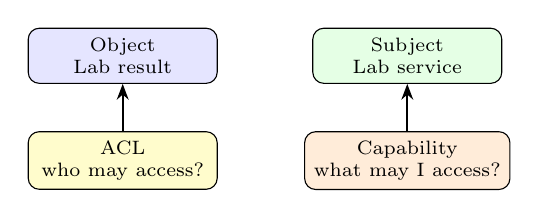
\begin{tikzpicture}[
    node distance=0.6cm and 1.2cm,
    box/.style={draw, rounded corners, align=center, minimum width=2.4cm, minimum height=0.7cm, font=\scriptsize},
    link/.style={-{Stealth[length=2mm]}, thick}
]
\node[box, fill=blue!10] (obj) {Object\\Lab result};
\node[box, below=of obj, fill=yellow!20] (acl) {ACL\\who may access?};
\node[box, right=of obj, fill=green!10] (subj) {Subject\\Lab service};
\node[box, below=of subj, fill=orange!15] (cap) {Capability\\what may I access?};
\draw[link] (acl) -- (obj);
\draw[link] (cap) -- (subj);
\end{tikzpicture}
\end{center}

\begin{block}{Trade-off}
ACLs make it easy to ask who can access one object. Capabilities make it easy to ask what one
subject can access.
\end{block}
\end{frame}

\begin{frame}[c]{Protecting Capabilities}
\begin{block}{Important}
A capability must be protected from forgery and tampering. Systems may store it in protected OS
memory or use cryptographic tokens such as message authentication codes.
\end{block}

\begin{exampleblock}{Hospital example}
If a lab device can forge a capability token, it might send results for departments it should not
serve. Signed or MAC-protected tokens make that harder.
\end{exampleblock}
\end{frame}

\begin{frame}[c]{Notebook: DAC Toy Model}
\begin{block}{Practical example}
Open \texttt{lesson-03/examples/01\_dac\_toy\_model.ipynb} after the DAC section.
\end{block}

\begin{exampleblock}{What students should notice}
The notebook represents the same hospital policy as an access matrix and as ACLs, then shows how
delegation changes a decision.
\end{exampleblock}

\begin{block}{Important}
This is only a teaching model. Real systems usually provide DAC or ACL mechanisms already;
administrators decide the sharing policy and review it.
\end{block}
\end{frame}

\begin{frame}[c]{Recap: DAC}
\begin{block}{Takeaways}
\begin{itemize}
    \item DAC decisions are based on identity and assigned rights.
    \item Delegation is powerful but can spread access too widely.
    \item Access matrices are conceptual; ACLs and capabilities are practical decompositions.
    \item Capability integrity is essential in distributed systems.
\end{itemize}
\end{block}
\end{frame}

\section{Mandatory Access Control}
\sectiontitleframe{Mandatory Access Control}

\begin{frame}[c]{Section Context: MAC}
\begin{block}{What we are talking about}
\textbf{Mandatory Access Control} uses centrally enforced labels and clearances. Users cannot
simply delegate access to others when the labels do not permit it.
\end{block}

\begin{exampleblock}{Hospital lens}
Some clinical data may need stronger controls than ordinary role permissions: psychiatric notes,
VIP records, infectious-disease investigations, or research datasets under strict agreements.
\end{exampleblock}
\end{frame}

\begin{frame}[c]{Labels and Clearances}
\begin{block}{Concept}
Objects receive \textbf{security labels} describing sensitivity. Subjects receive
\textbf{clearances} describing what sensitivity they may access.
\end{block}

\begin{exampleblock}{Hospital example}
A note labelled ``restricted mental health'' may require a clinician clearance for that department
and a valid care relationship.
\end{exampleblock}
\end{frame}

\begin{frame}[c]{Dominance}
\begin{block}{Concept}
A subject may read an object only if the subject \textbf{dominates} the object: the subject has a
sufficient rank and the required compartments.
\end{block}

\begin{exampleblock}{Hospital example}
A senior infectious-disease physician may access records tagged for the outbreak investigation.
A cardiologist with a higher clinical title but without that compartment may still be denied.
\end{exampleblock}
\end{frame}

\begin{frame}[c]{Rank and Compartment}
\begin{block}{Two dimensions}
\textbf{Rank} expresses level of sensitivity. \textbf{Compartment} expresses membership in a
specific project, ward, study, or controlled domain.
\end{block}

\begin{exampleblock}{Hospital example}
\texttt{<restricted; oncology-trial>} requires enough sensitivity clearance and membership in the
oncology-trial compartment.
\end{exampleblock}
\end{frame}

\begin{frame}[c]{Scheme: MAC Decision}
\begin{center}
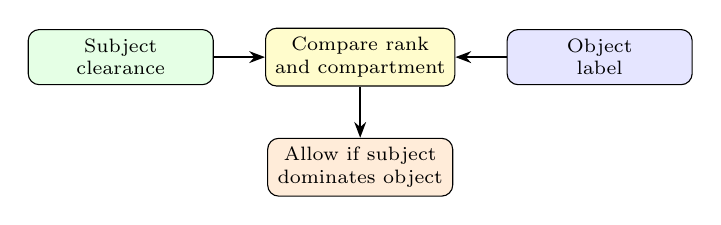
\begin{tikzpicture}[
    node distance=0.65cm,
    box/.style={draw, rounded corners, align=center, minimum width=2.35cm, minimum height=0.7cm, font=\scriptsize},
    link/.style={-{Stealth[length=2mm]}, thick}
]
\node[box, fill=green!10] (subject) {Subject\\clearance};
\node[box, right=of subject, fill=yellow!20] (compare) {Compare rank\\and compartment};
\node[box, right=of compare, fill=blue!10] (object) {Object\\label};
\node[box, below=of compare, fill=orange!15] (decision) {Allow if subject\\dominates object};
\draw[link] (subject) -- (compare);
\draw[link] (object) -- (compare);
\draw[link] (compare) -- (decision);
\end{tikzpicture}
\end{center}

\begin{block}{Important}
MAC is useful when the organization must prevent unauthorized information flows, even if an
individual user would like to share the resource.
\end{block}
\end{frame}

\begin{frame}[c]{MAC Example Decisions}
\begin{center}
\scriptsize
\renewcommand{\arraystretch}{1.2}
\begin{tabular}{p{0.28\textwidth} p{0.28\textwidth} p{0.28\textwidth}}
\toprule
Subject clearance & Object label & Decision \\
\midrule
\texttt{<restricted; oncology>} & \texttt{<confidential; oncology>} & Allow \\
\texttt{<restricted; cardiology>} & \texttt{<confidential; oncology>} & Deny: wrong compartment \\
\texttt{<internal; oncology>} & \texttt{<restricted; oncology>} & Deny: rank too low \\
\bottomrule
\end{tabular}
\end{center}

\begin{exampleblock}{Hospital example}
The decision is not just seniority. The subject must have both enough level and the right clinical
or project compartment.
\end{exampleblock}
\end{frame}

\begin{frame}[c]{Notebook: MAC Toy Model}
\begin{block}{Practical example}
Open \texttt{lesson-03/examples/02\_mac\_toy\_model.ipynb} after the MAC section.
\end{block}

\begin{exampleblock}{What students should notice}
The notebook compares subject clearances with object labels. Changing a label can deny access
without changing the user's identity.
\end{exampleblock}

\begin{block}{Important}
This is only a teaching model. Real MAC enforcement is supplied by platforms such as operating
systems, database engines, or specialized security products.
\end{block}
\end{frame}

\begin{frame}[c]{Recap: MAC}
\begin{block}{Takeaways}
\begin{itemize}
    \item MAC uses labels on objects and clearances on subjects.
    \item Access depends on rank and compartment.
    \item Users cannot freely delegate labelled information.
    \item MAC is strict, powerful, and administratively demanding.
\end{itemize}
\end{block}
\end{frame}

\section{Role-Based Access Control}
\sectiontitleframe{Role-Based Access Control}

\begin{frame}[c]{Section Context: RBAC}
\begin{block}{What we are talking about}
\textbf{Role-Based Access Control} assigns permissions to roles rather than directly to individual
users. Users receive roles according to their responsibilities.
\end{block}

\begin{exampleblock}{Hospital lens}
Hospitals have many users and many resources, but a smaller set of job functions: ward nurse,
attending physician, lab technician, pharmacist, registrar, auditor, and system administrator.
\end{exampleblock}
\end{frame}

\begin{frame}[c]{Why RBAC Fits Organizations}
\begin{block}{Concept}
Users change often. Permissions attached to job functions change less often. RBAC reduces the
administrative burden by managing role assignments and role permissions separately.
\end{block}

\begin{exampleblock}{Hospital example}
When a new nurse joins the emergency department, IT assigns the ``ED nurse'' role instead of
manually granting every permission needed for triage, vitals, and documentation.
\end{exampleblock}
\end{frame}

\begin{frame}[c]{Scheme: RBAC Mapping}
\begin{center}
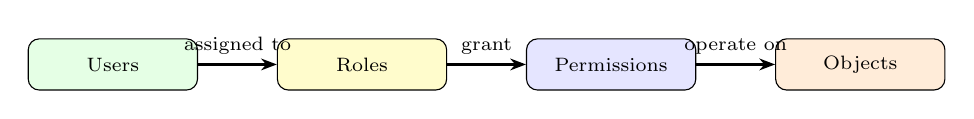
\begin{tikzpicture}[
    node distance=0.6cm and 1.0cm,
    box/.style={draw, rounded corners, align=center, minimum width=2.15cm, minimum height=0.65cm, font=\scriptsize},
    link/.style={-{Stealth[length=2mm]}, thick}
]
\node[box, fill=green!10] (users) {Users};
\node[box, right=of users, fill=yellow!20] (roles) {Roles};
\node[box, right=of roles, fill=blue!10] (perms) {Permissions};
\node[box, right=of perms, fill=orange!15] (objects) {Objects};
\draw[link] (users) -- node[above,font=\scriptsize]{assigned to} (roles);
\draw[link] (roles) -- node[above,font=\scriptsize]{grant} (perms);
\draw[link] (perms) -- node[above,font=\scriptsize]{operate on} (objects);
\end{tikzpicture}
\end{center}

\begin{block}{Reading the scheme}
RBAC answers access requests through the active role, not only the user's personal identity.
\end{block}
\end{frame}

\begin{frame}[c]{RBAC0: Core Model}
\begin{block}{Core entities}
RBAC0 contains \textbf{users}, \textbf{roles}, \textbf{permissions}, and \textbf{sessions}. A
session maps a user to the roles activated for a specific task.
\end{block}

\begin{exampleblock}{Hospital example}
Dr. Rossi may have both ``cardiologist'' and ``researcher'' roles, but during a clinical session only
the cardiologist role should be active.
\end{exampleblock}
\end{frame}

\begin{frame}[c]{Sessions Matter}
\begin{block}{Concept}
A user may be assigned multiple roles, but a session should activate only the roles needed now.
This supports least privilege.
\end{block}

\begin{exampleblock}{Hospital example}
The same physician does not need research-export permissions while prescribing medication in the
emergency department.
\end{exampleblock}
\end{frame}

\begin{frame}[c]{RBAC1: Role Hierarchies}
\begin{block}{Concept}
RBAC1 adds role hierarchies. A senior role can inherit permissions from subordinate roles, reducing
duplication.
\end{block}

\begin{exampleblock}{Hospital example}
``Senior pharmacist'' inherits normal pharmacist permissions and adds authority to approve high-risk
medication substitutions.
\end{exampleblock}
\end{frame}

\begin{frame}[c]{Scheme: Role Hierarchy}
\begin{center}
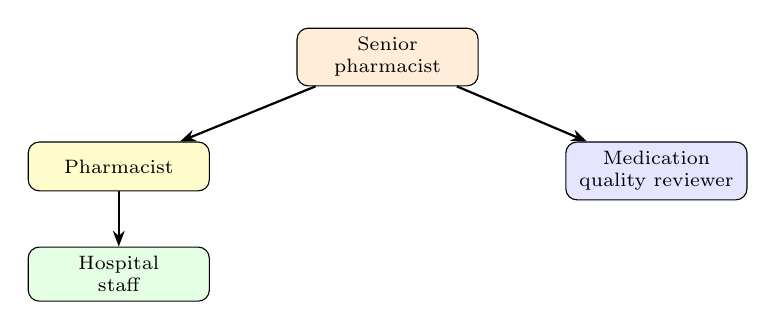
\begin{tikzpicture}[
    node distance=0.7cm and 1.1cm,
    box/.style={draw, rounded corners, align=center, minimum width=2.3cm, minimum height=0.62cm, font=\scriptsize},
    link/.style={-{Stealth[length=2mm]}, thick}
]
\node[box, fill=orange!15] (senior) {Senior\\pharmacist};
\node[box, below left=of senior, fill=yellow!20] (pharm) {Pharmacist};
\node[box, below right=of senior, fill=blue!10] (quality) {Medication\\quality reviewer};
\node[box, below=of pharm, fill=green!10] (staff) {Hospital\\staff};
\draw[link] (senior) -- (pharm);
\draw[link] (senior) -- (quality);
\draw[link] (pharm) -- (staff);
\end{tikzpicture}
\end{center}

\begin{block}{Reading the scheme}
Hierarchies simplify shared permissions, but inherited privileges must still respect least
privilege.
\end{block}
\end{frame}

\begin{frame}[c]{RBAC2: Constraints}
\begin{block}{Concept}
RBAC2 adds constraints that express organizational policy, such as mutually exclusive roles,
cardinality limits, and prerequisite roles.
\end{block}

\begin{exampleblock}{Hospital example}
The same user should not both request and approve creation of a privileged EHR administrator
account.
\end{exampleblock}
\end{frame}

\begin{frame}[c]{Mutually Exclusive Roles}
\begin{block}{Concept}
Mutual exclusion prevents one user or one session from holding roles that should not be combined.
This supports separation of duty.
\end{block}

\begin{exampleblock}{Hospital example}
A user may not be both ``controlled-drug inventory clerk'' and ``controlled-drug audit approver''
for the same reporting period.
\end{exampleblock}
\end{frame}

\begin{frame}[c]{Cardinality and Prerequisites}
\begin{block}{Concept}
\textbf{Cardinality} limits how many users may hold a role or how many roles may grant a privilege.
\textbf{Prerequisite roles} require a user to hold one role before receiving another.
\end{block}

\begin{exampleblock}{Hospital example}
Only two users may hold the ``break-glass policy administrator'' role. A clinician must first be an
attending physician before becoming an ICU attending.
\end{exampleblock}
\end{frame}

\begin{frame}[c]{RBAC3 and NIST RBAC}
\begin{block}{Concept}
NIST standardized RBAC around core RBAC, hierarchical RBAC, and separation-of-duty relations
\cite{nist_rbac}. The model also describes administrative, system-support, and review functions.
\end{block}

\begin{exampleblock}{Hospital example}
Administrators create roles and assignments; the EHR checks permissions during sessions; auditors
review which users, roles, and permissions exist.
\end{exampleblock}
\end{frame}

\begin{frame}[c]{Static and Dynamic Separation of Duty}
\begin{block}{Two controls}
\textbf{Static separation of duty} prevents conflicting role assignments. \textbf{Dynamic
separation of duty} prevents conflicting roles from being active in the same session.
\end{block}

\begin{exampleblock}{Hospital example}
A person may be assigned both clinician and researcher roles, but cannot activate both when
exporting identifiable clinical data for a study.
\end{exampleblock}
\end{frame}

\begin{frame}[c]{Notebook: RBAC Toy Model}
\begin{block}{Practical example}
Open \texttt{lesson-03/examples/03\_rbac\_toy\_model.ipynb} after the RBAC section.
\end{block}

\begin{exampleblock}{What students should notice}
The notebook separates users, roles, permissions, and sessions. It shows that changing the active
session can change the access decision.
\end{exampleblock}

\begin{block}{Important}
This is only a teaching model. In real EHRs and identity platforms, administrators design roles,
assign users, set constraints, and review access.
\end{block}
\end{frame}

\begin{frame}[c]{Recap: RBAC}
\begin{block}{Takeaways}
\begin{itemize}
    \item RBAC assigns permissions to roles, then users to roles.
    \item Sessions activate only the roles needed for the current task.
    \item Hierarchies reduce duplication but can accidentally accumulate privilege.
    \item Constraints express least privilege and separation of duty.
\end{itemize}
\end{block}
\end{frame}

\section{Choosing and Combining Models}
\sectiontitleframe{Choosing and Combining Models}

\begin{frame}[c]{Section Context: Choosing Models}
\begin{block}{What we are talking about}
DAC, MAC, and RBAC are not mutually exclusive. Real healthcare systems often combine them across
operating systems, applications, databases, devices, and networks.
\end{block}

\begin{exampleblock}{Hospital lens}
An EHR can use RBAC for clinical roles, DAC-like ACLs for document sharing, MAC-like labels for
highly sensitive notes, and audit rules for accountability.
\end{exampleblock}
\end{frame}

\begin{frame}[c]{Comparison}
\begin{center}
\scriptsize
\renewcommand{\arraystretch}{1.25}
\begin{tabular}{@{}>{\bfseries}p{0.16\textwidth} p{0.23\textwidth} p{0.23\textwidth} p{0.22\textwidth}@{}}
\toprule
Model & Main basis & Strength & Main caution \\
\midrule
DAC & Identity and delegated rights & Flexible sharing & Access can spread too widely \\
MAC & Labels and clearances & Strong information-flow control & Rigid and costly to administer \\
RBAC & Organizational roles & Scales with job functions & Role explosion and inherited privilege \\
\bottomrule
\end{tabular}
\end{center}
\end{frame}

\begin{frame}[c]{Notebook: Comparing Models}
\begin{block}{Practical example}
Open \texttt{lesson-03/examples/04\_compare\_models.ipynb} after the comparison slide.
\end{block}

\begin{exampleblock}{What students should notice}
The same request can be allowed by DAC, denied by MAC, and allowed by RBAC, because each model asks
a different policy question.
\end{exampleblock}

\begin{block}{Important}
The notebooks explain concepts, not production engineering. In practice, system administrators
select and configure the access-control policy provided by the real system.
\end{block}
\end{frame}

\begin{frame}[c]{Emergency Access}
\begin{block}{Concept}
Healthcare sometimes needs \textbf{break-glass} access: temporary emergency access that bypasses
normal restrictions but creates strong audit evidence.
\end{block}

\begin{exampleblock}{Hospital example}
An emergency physician can open an unconscious patient's allergy history outside normal assignment
rules. The access is logged, justified, time-limited, and reviewed.
\end{exampleblock}
\end{frame}

\begin{frame}[c]{Access Control and GDPR}
\begin{block}{Connection}
Access control supports confidentiality, integrity, availability, accountability, and data
minimization. It helps ensure that personal health data is processed only by authorized people for
authorized purposes.
\end{block}

\begin{exampleblock}{Hospital example}
Audit logs and role assignments help St. Isidore demonstrate that access to patient records is
controlled, reviewed, and aligned with operational necessity.
\end{exampleblock}
\end{frame}

\begin{frame}[c]{Final Recap}
\begin{block}{What to remember}
\begin{itemize}
    \item Access control mediates use of protected resources.
    \item AAA separates identity proof, permission decisions, and accountability.
    \item Good policy design includes least privilege, separation of duty, conflict handling, and administration.
    \item DAC, MAC, and RBAC provide different ways to model and enforce access.
    \item Healthcare systems usually combine models because care workflows are complex.
\end{itemize}
\end{block}
\end{frame}

\begin{frame}[allowframebreaks]{References}
\bibliographystyle{apalike-AMS}
\bibliography{main}
\end{frame}

\end{document}
